% !TEX root = ../eval.tex

\section{Unbalanced aggregation}%
\label{sec:unbalanced_aggregation}

The baseline specification relies on a panel balanced in event time and
thus only includes users that have been exposed to treatment for at least 5
periods. Figure~\ref{fig:ub_comp} reproduces the baseline results in the left
panel and compares it with results based on the full sample.

As discussed in section 3.1.1 of \citet{callaway2021difference}, these two
approaches entail a trade-off. When using the full sample, the aggregated
parameters are a function of the weighted average treatment effects for each
group $l$ periods after treatment (which is what we want) as well as
compositional changes due to different groups being included for different
periods $l$ and different weights attached to these groups. While parameters
aggregated using a panel balanced in event time do not suffer from
compositional and weighting changes, but are calculated based on a smaller
number of groups.

As expected, using the full data reduces the size of the confidence intervals.
But the results are otherwise very similar.

\begin{figure}[h]
    \centering
    \caption{Balanced and unbalanced aggregation}%
    \label{fig:ub_comp}
    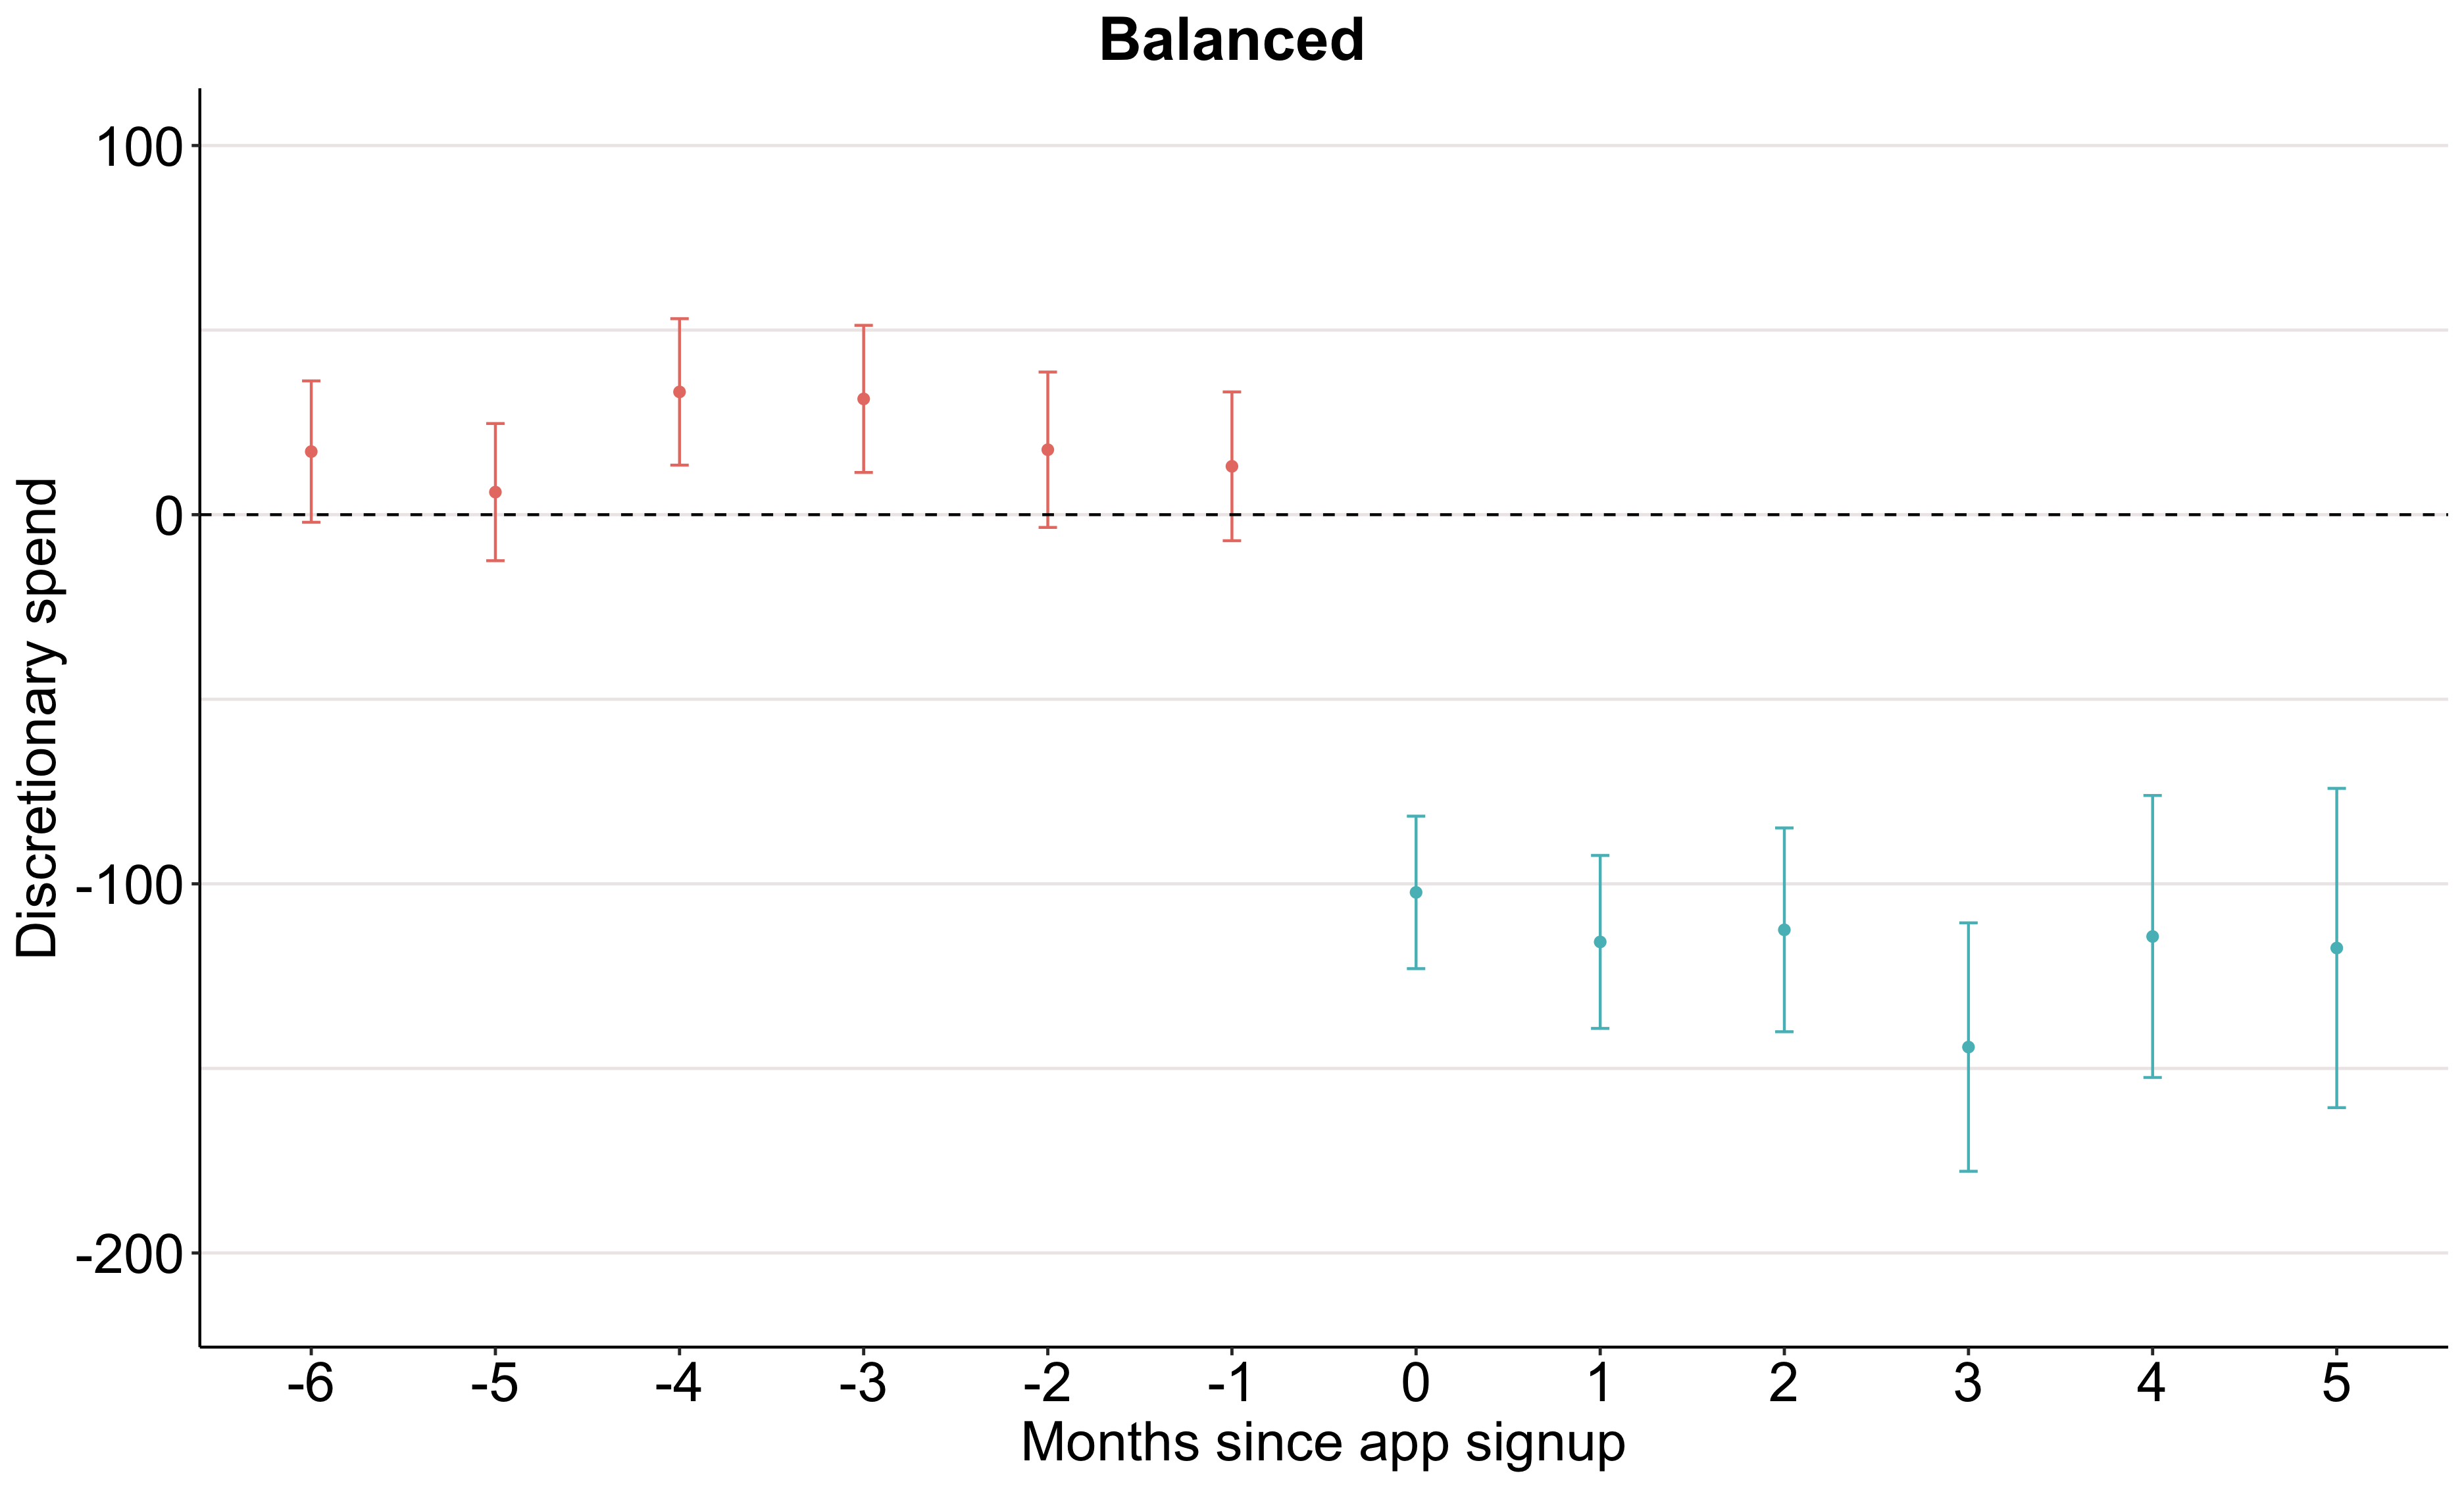
\includegraphics[width=.49\textwidth]{\figdir/dspend_cond_bal_es.png}
    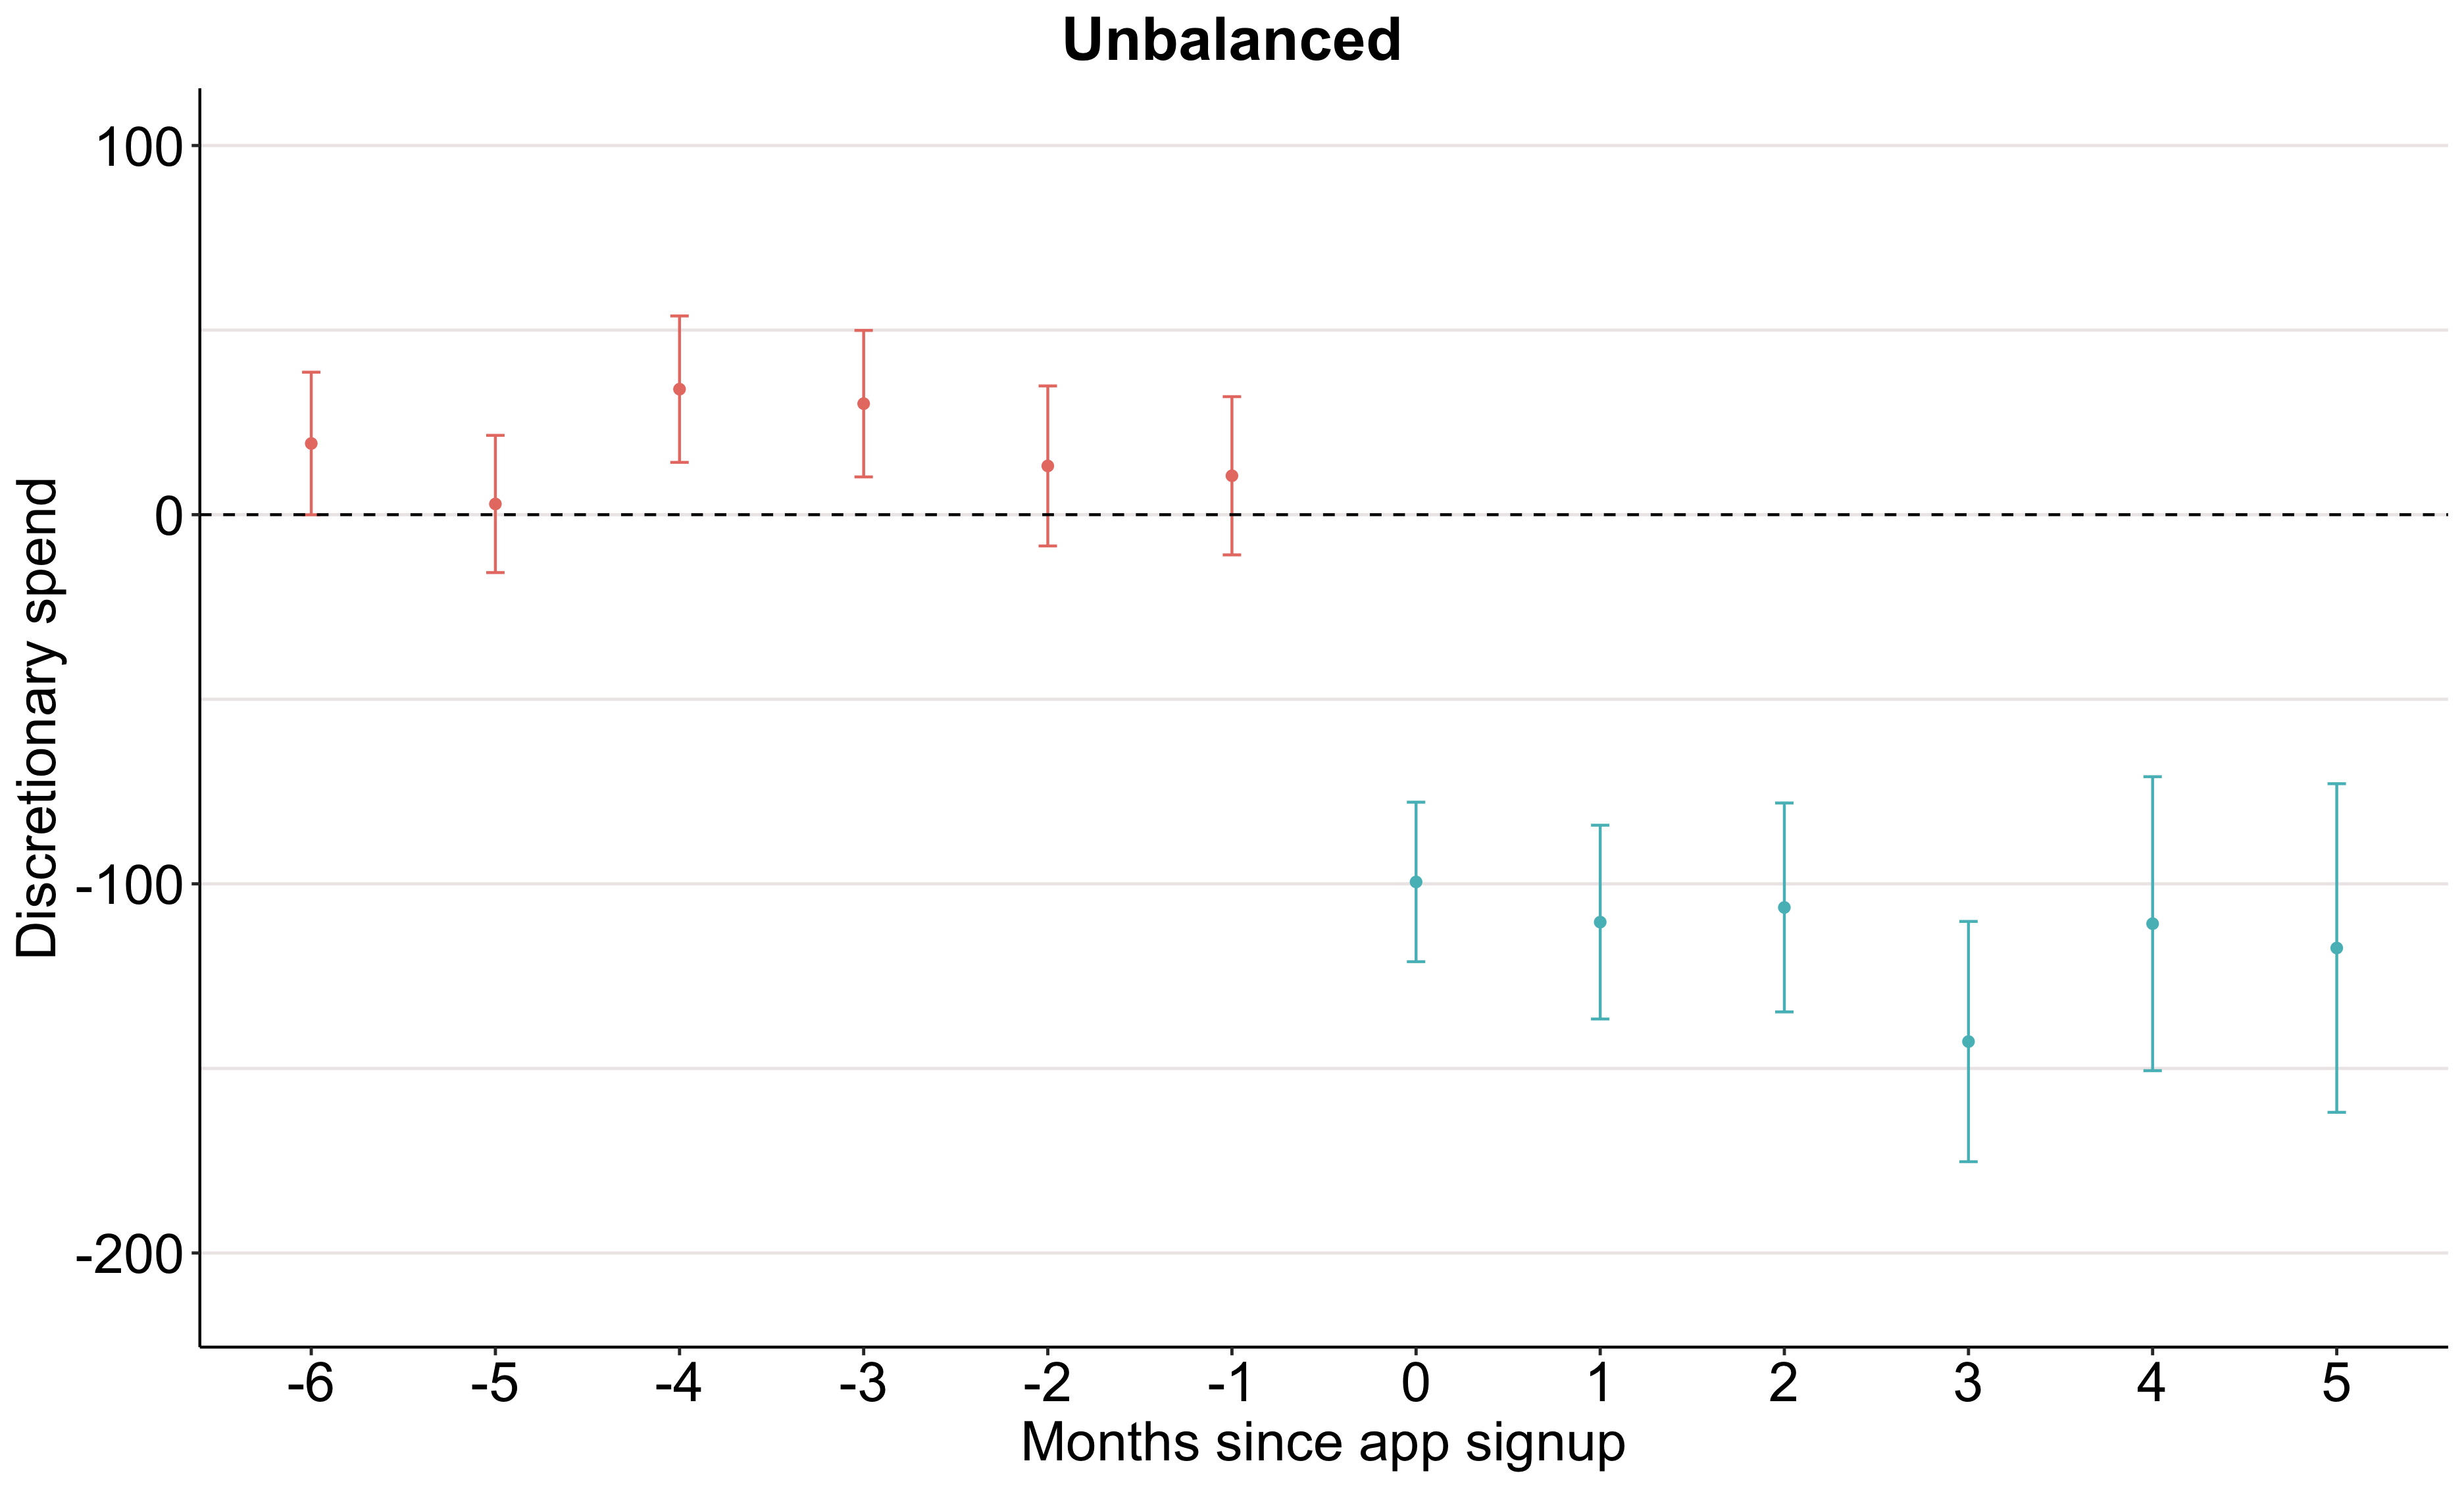
\includegraphics[width=.49\textwidth]{\figdir/dspend_cond_unbal_es.png}
    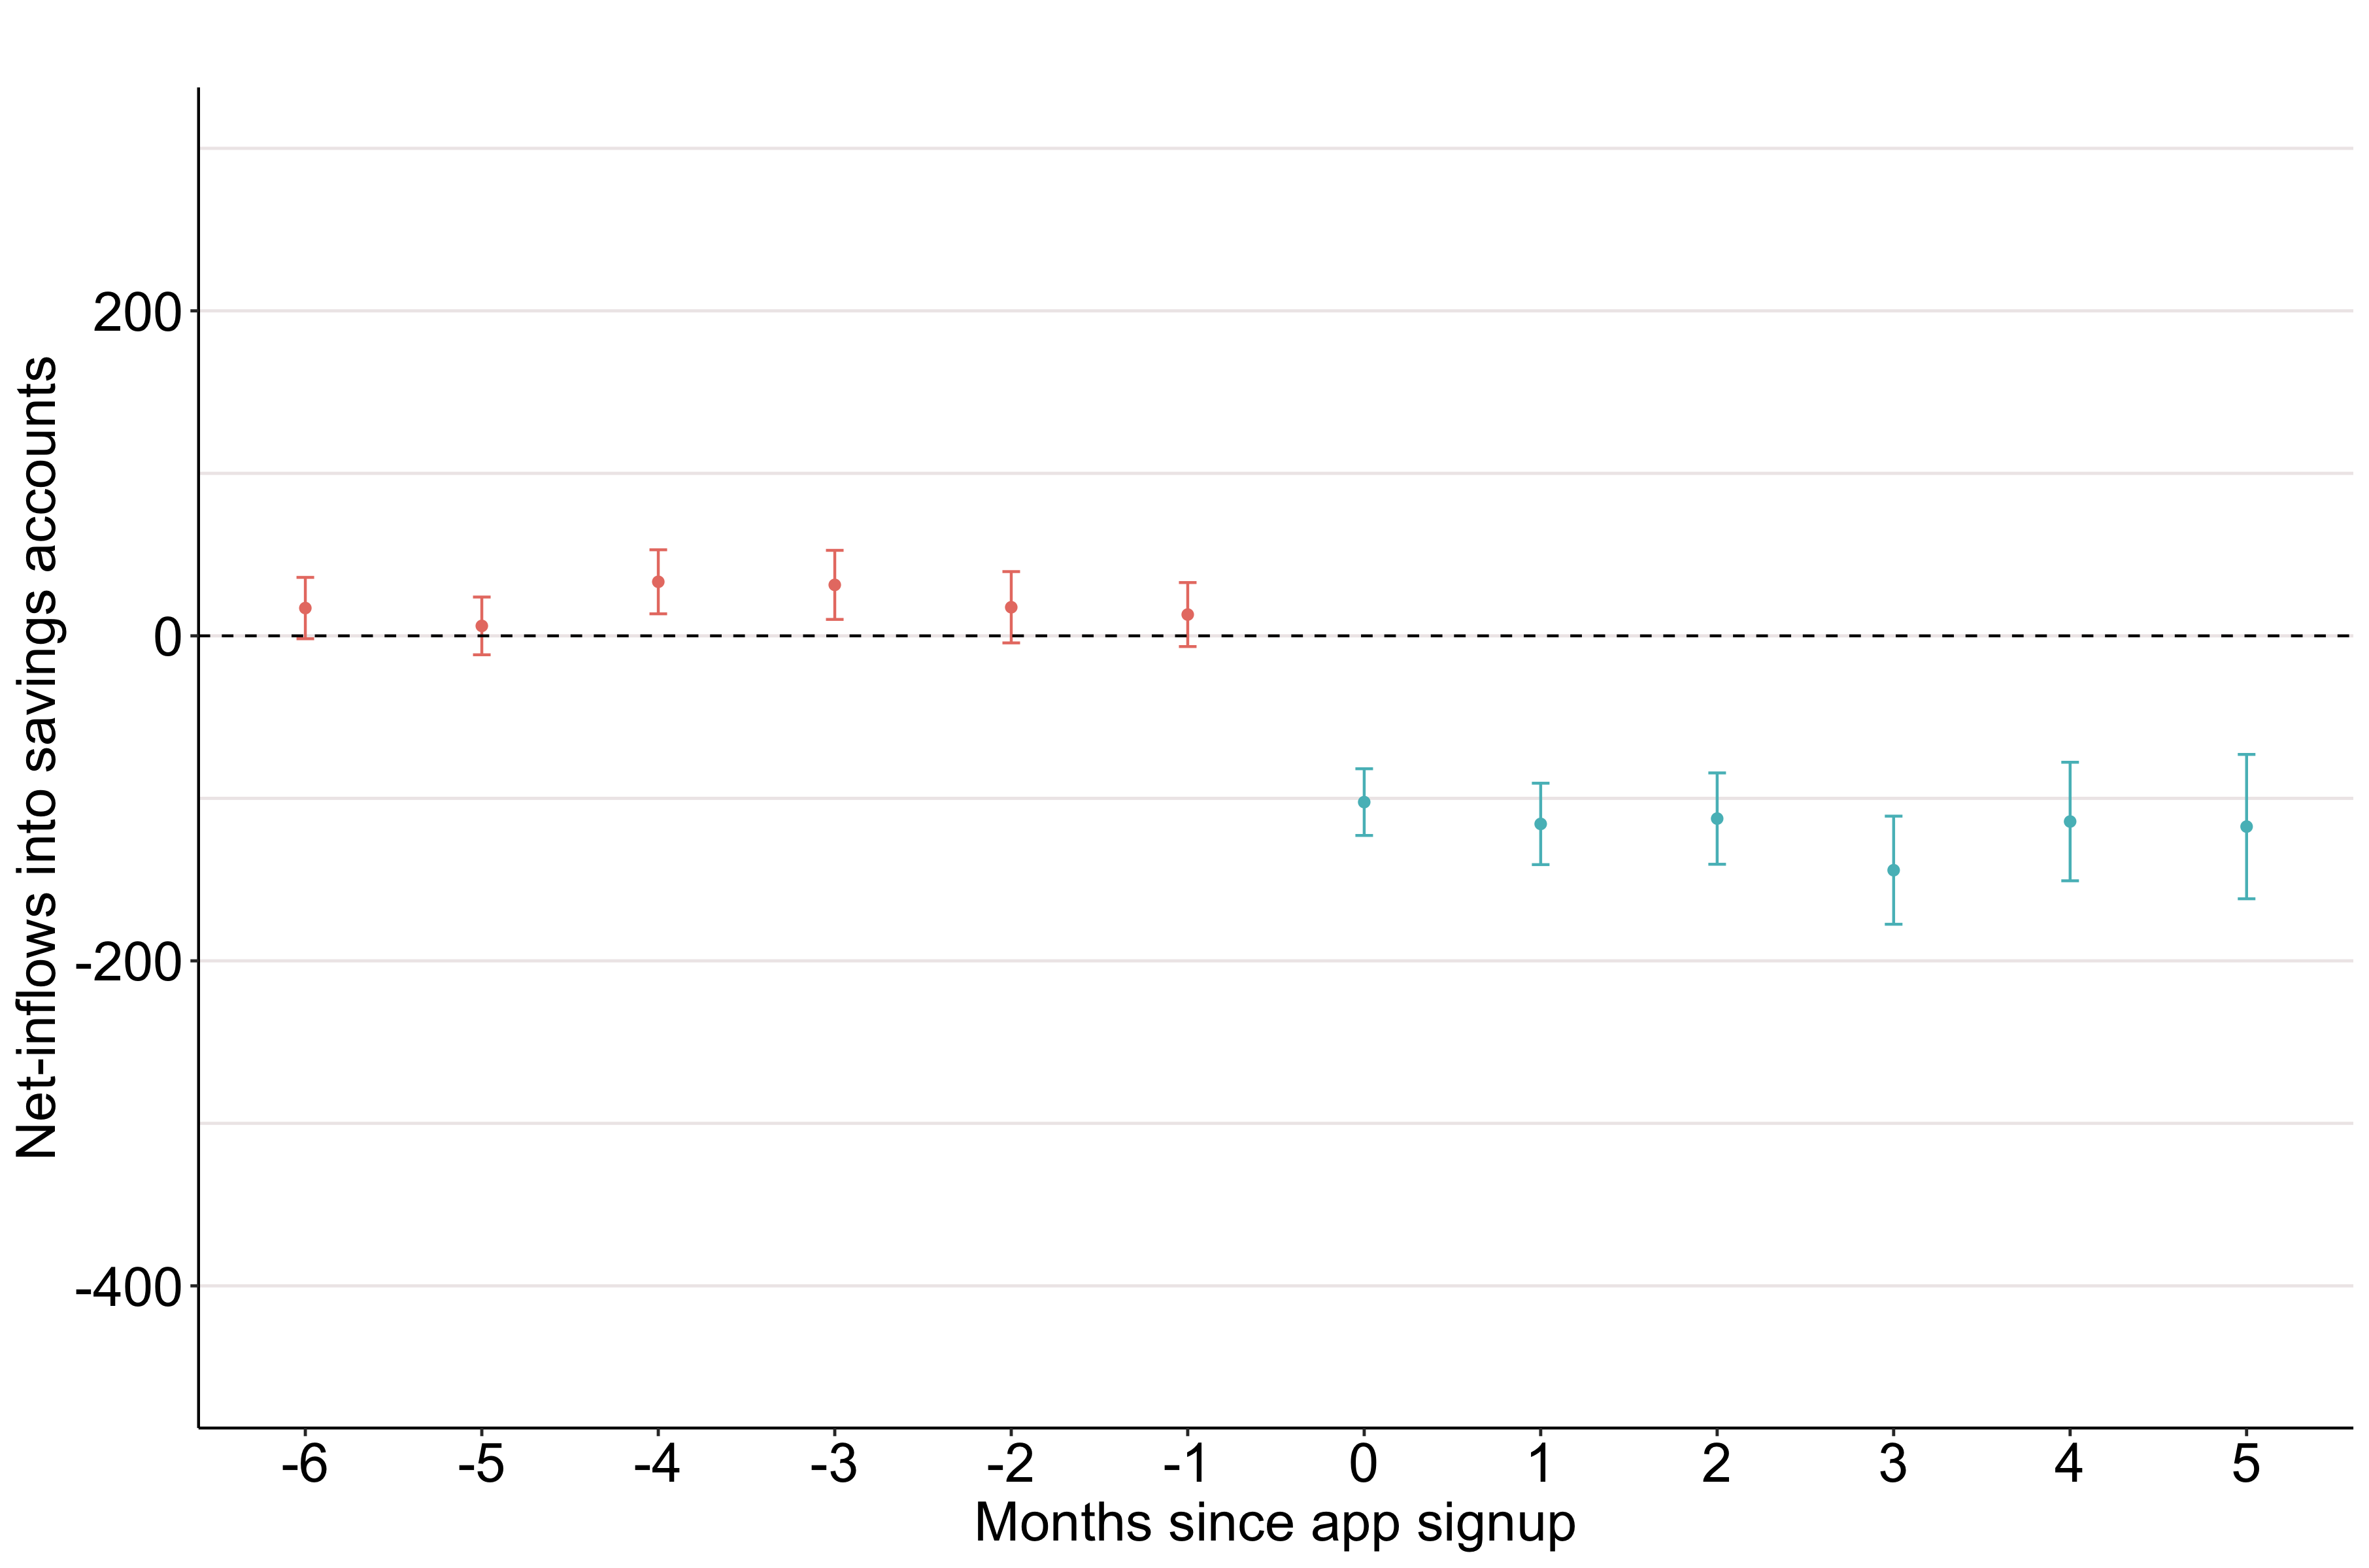
\includegraphics[width=.49\textwidth]{\figdir/netflows_cond_bal_es.png}
    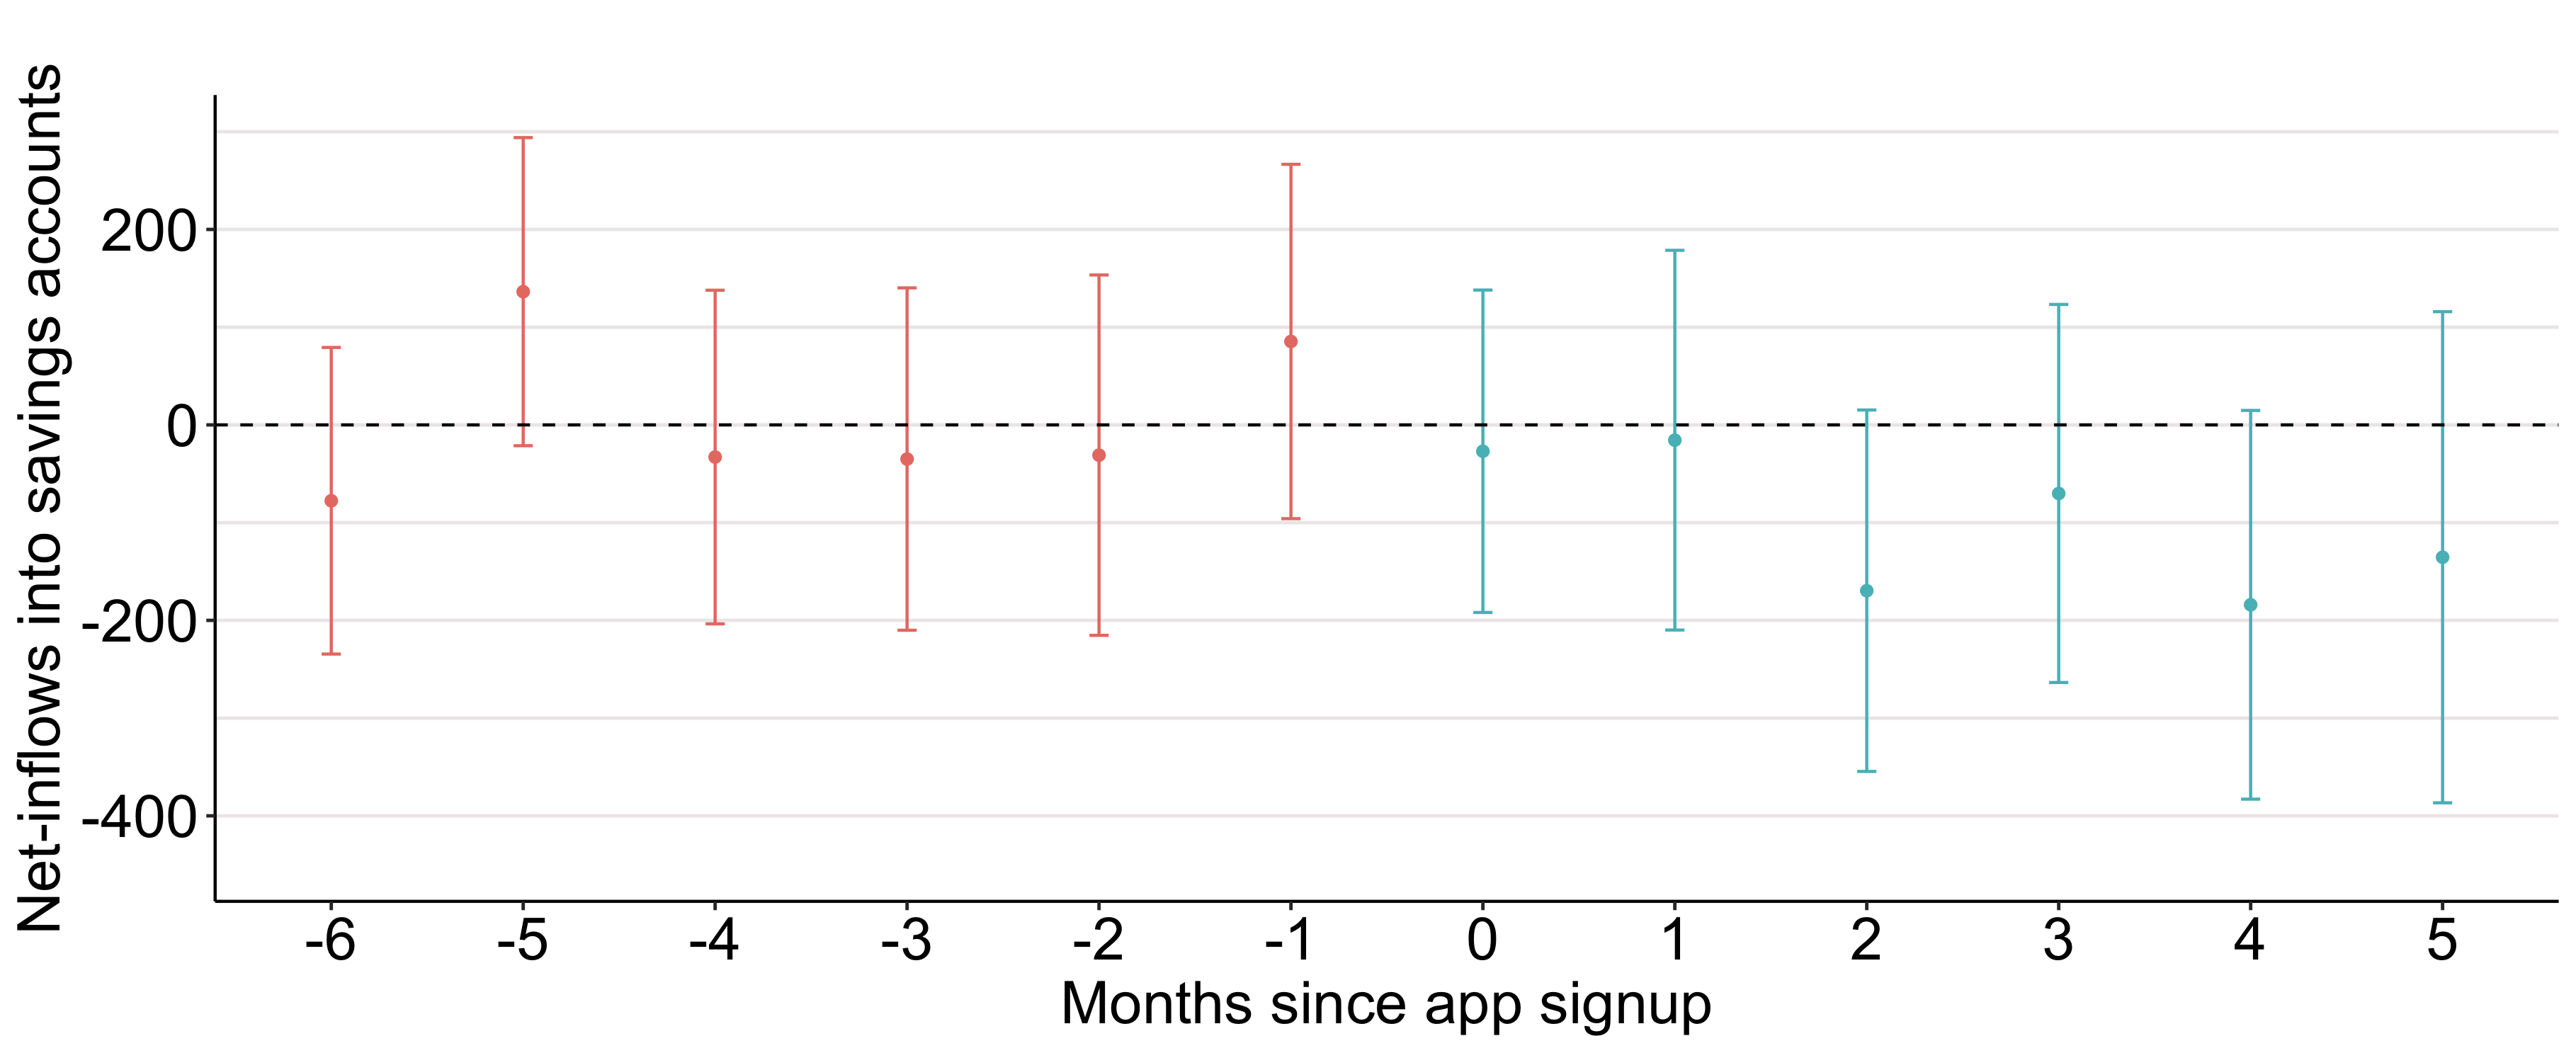
\includegraphics[width=.49\textwidth]{\figdir/netflows_cond_unbal_es.png}
    \fignote{\textwidth}{Main results based on balanced and unbalanced panels.
        Point estimates represent group-time average treatment effects
        aggregated to periods since treatment exposure, as defined in
        Section~\ref{sec:estimation}. Red lines represent point estimates and
        uniform 95\% confidence bands for pre-treatment periods allowing for
        clustering at the user level. If the null hypothesis that parallel
        trends hold in all periods is correct, these should be equal to zero.
        Blue lines provide similar information for post-treatment periods.}
\end{figure}



\section{Inflows and outflows}%
\label{sec:inflows_and_outflows}

The leftmost panel in Figure~\ref{fig:in_out_results} reproduces the results from
Figure~\ref{fig:main_results} for net inflows into savings accounts using the
conditional parallel trends assumption for reference, and decomposes these
net-inflows into inflows (middle) and outflows (bottom). We can see that
net-inflows remain unchanged because both inflows and outflows remain
unchanged and not because a change in inflows if offset by a commensurate
change in outflows.

\begin{figure}[H]
    \centering
    \caption{Decomposing net-inflows into inflows and outflows}%
    \label{fig:in_out_results}
    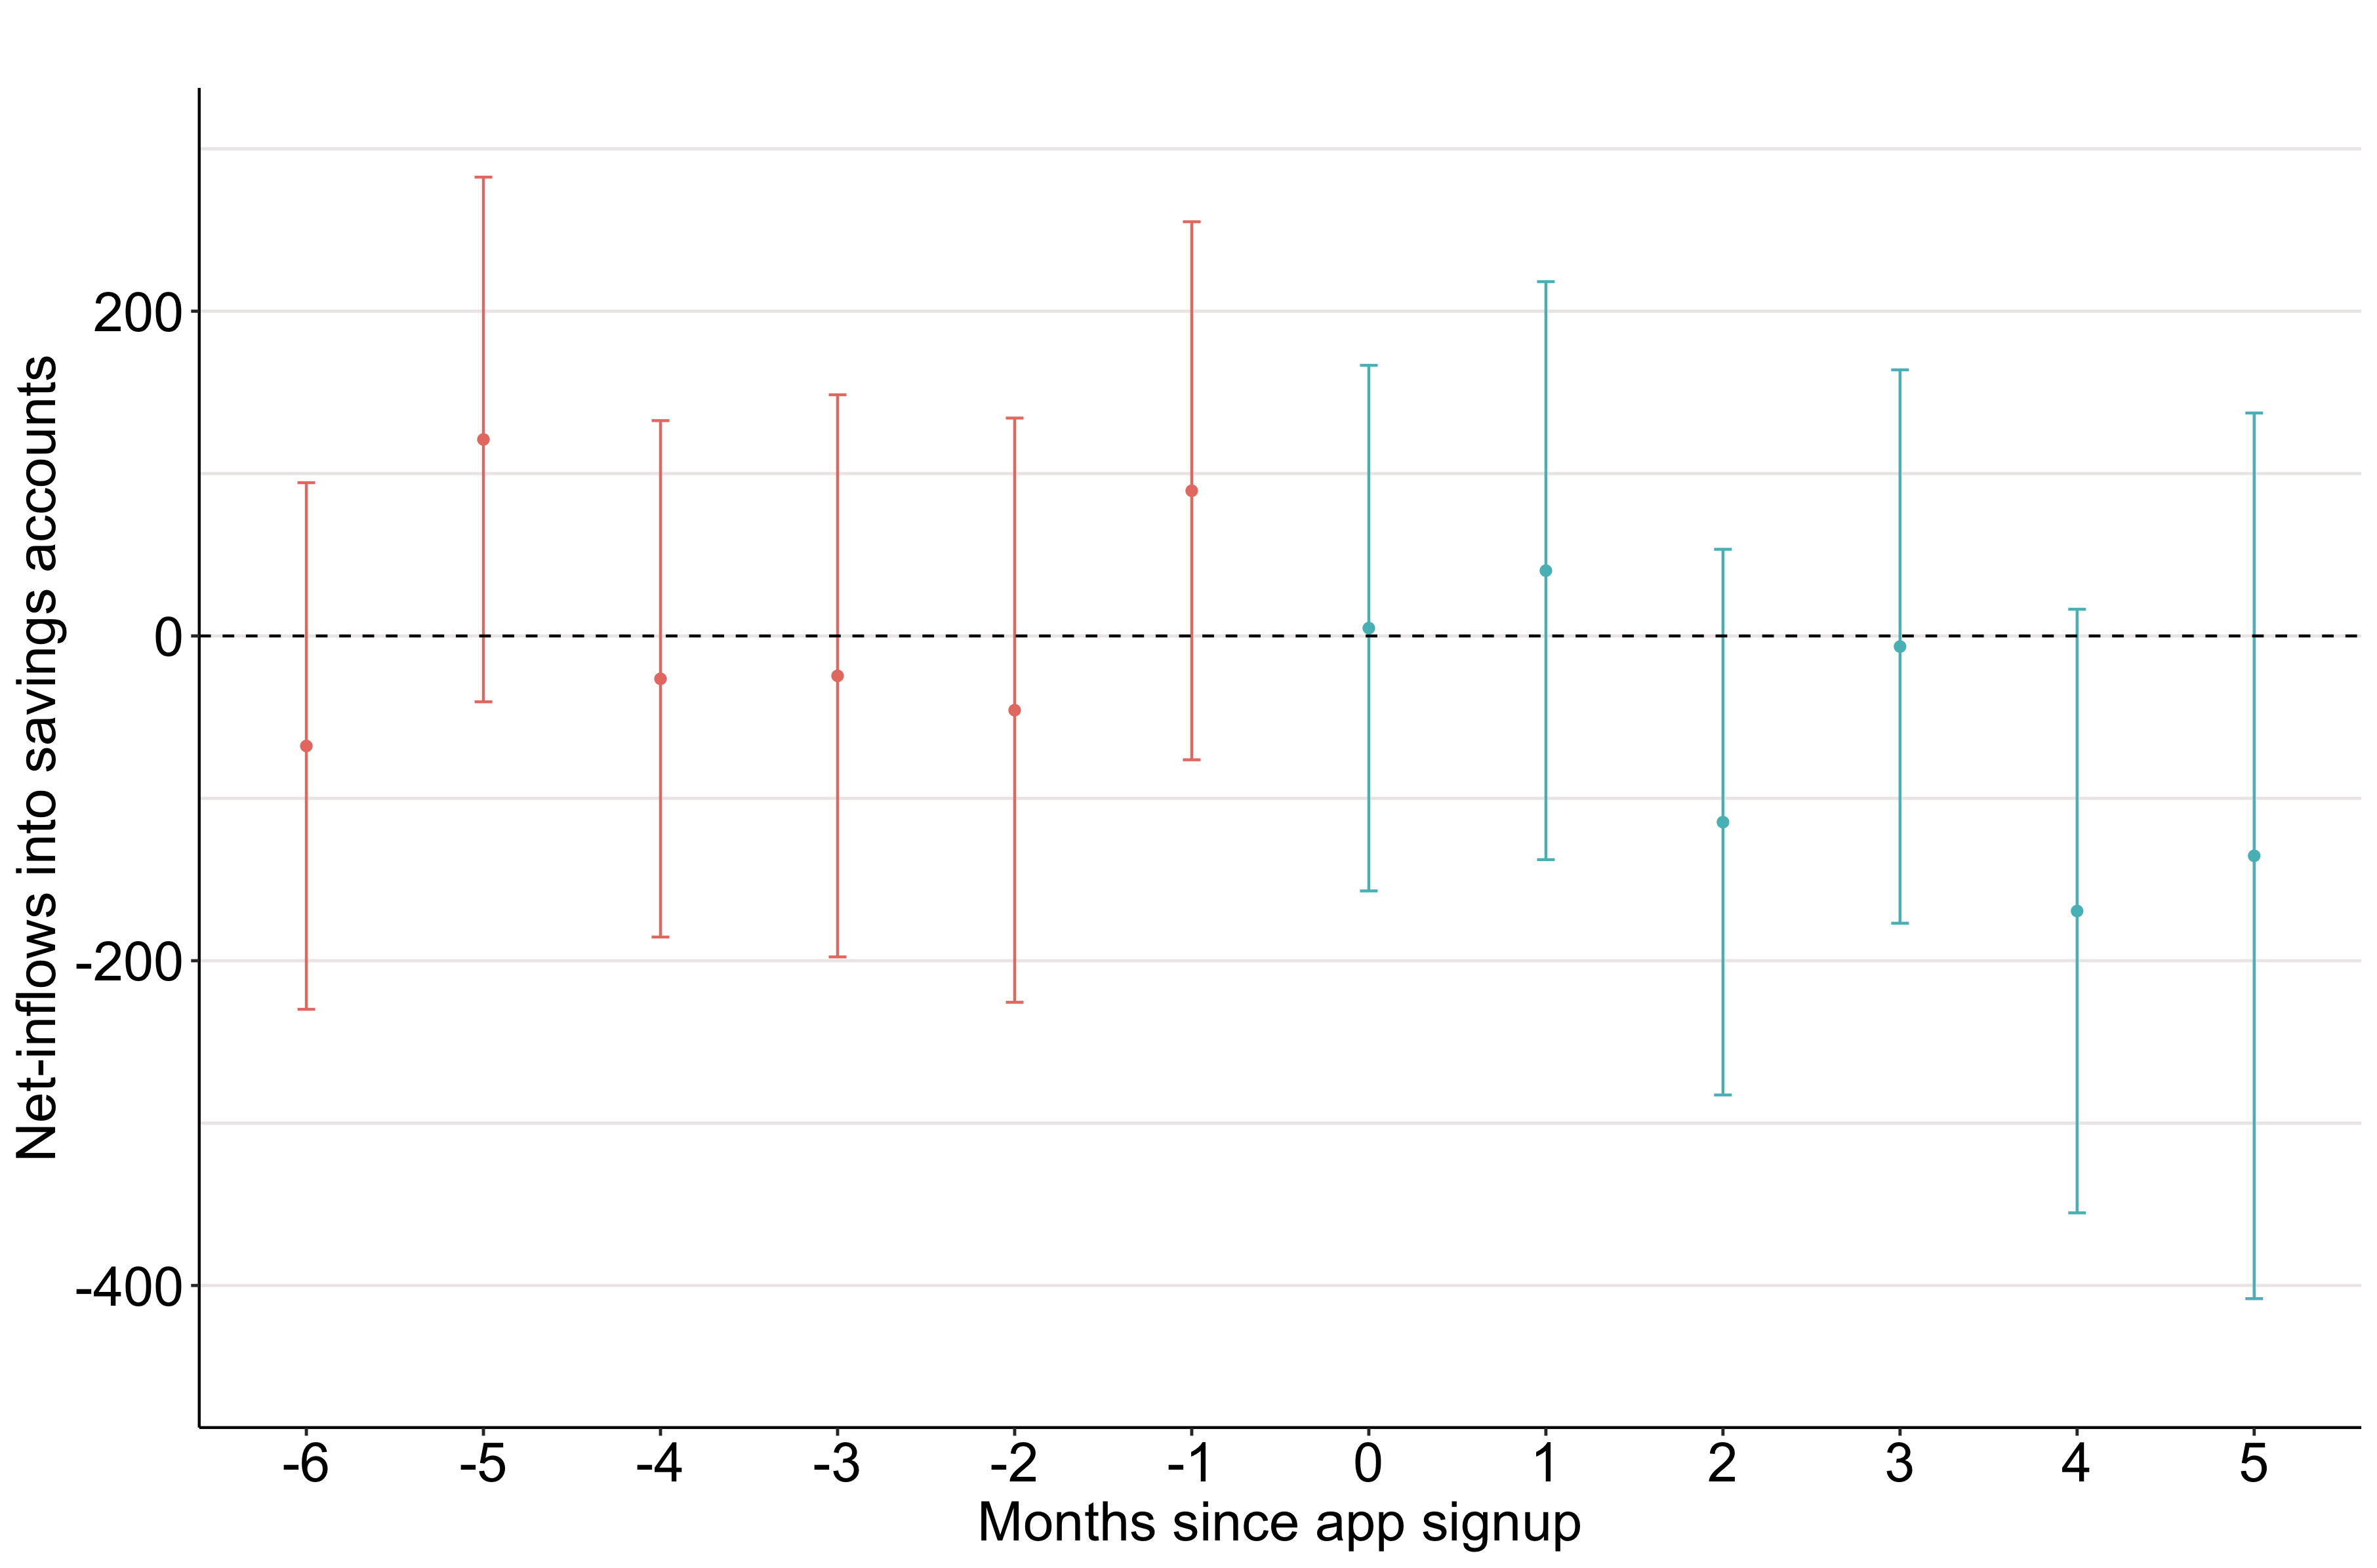
\includegraphics[width=.7\textwidth]{\figdir/netflows_cond_es.png}
    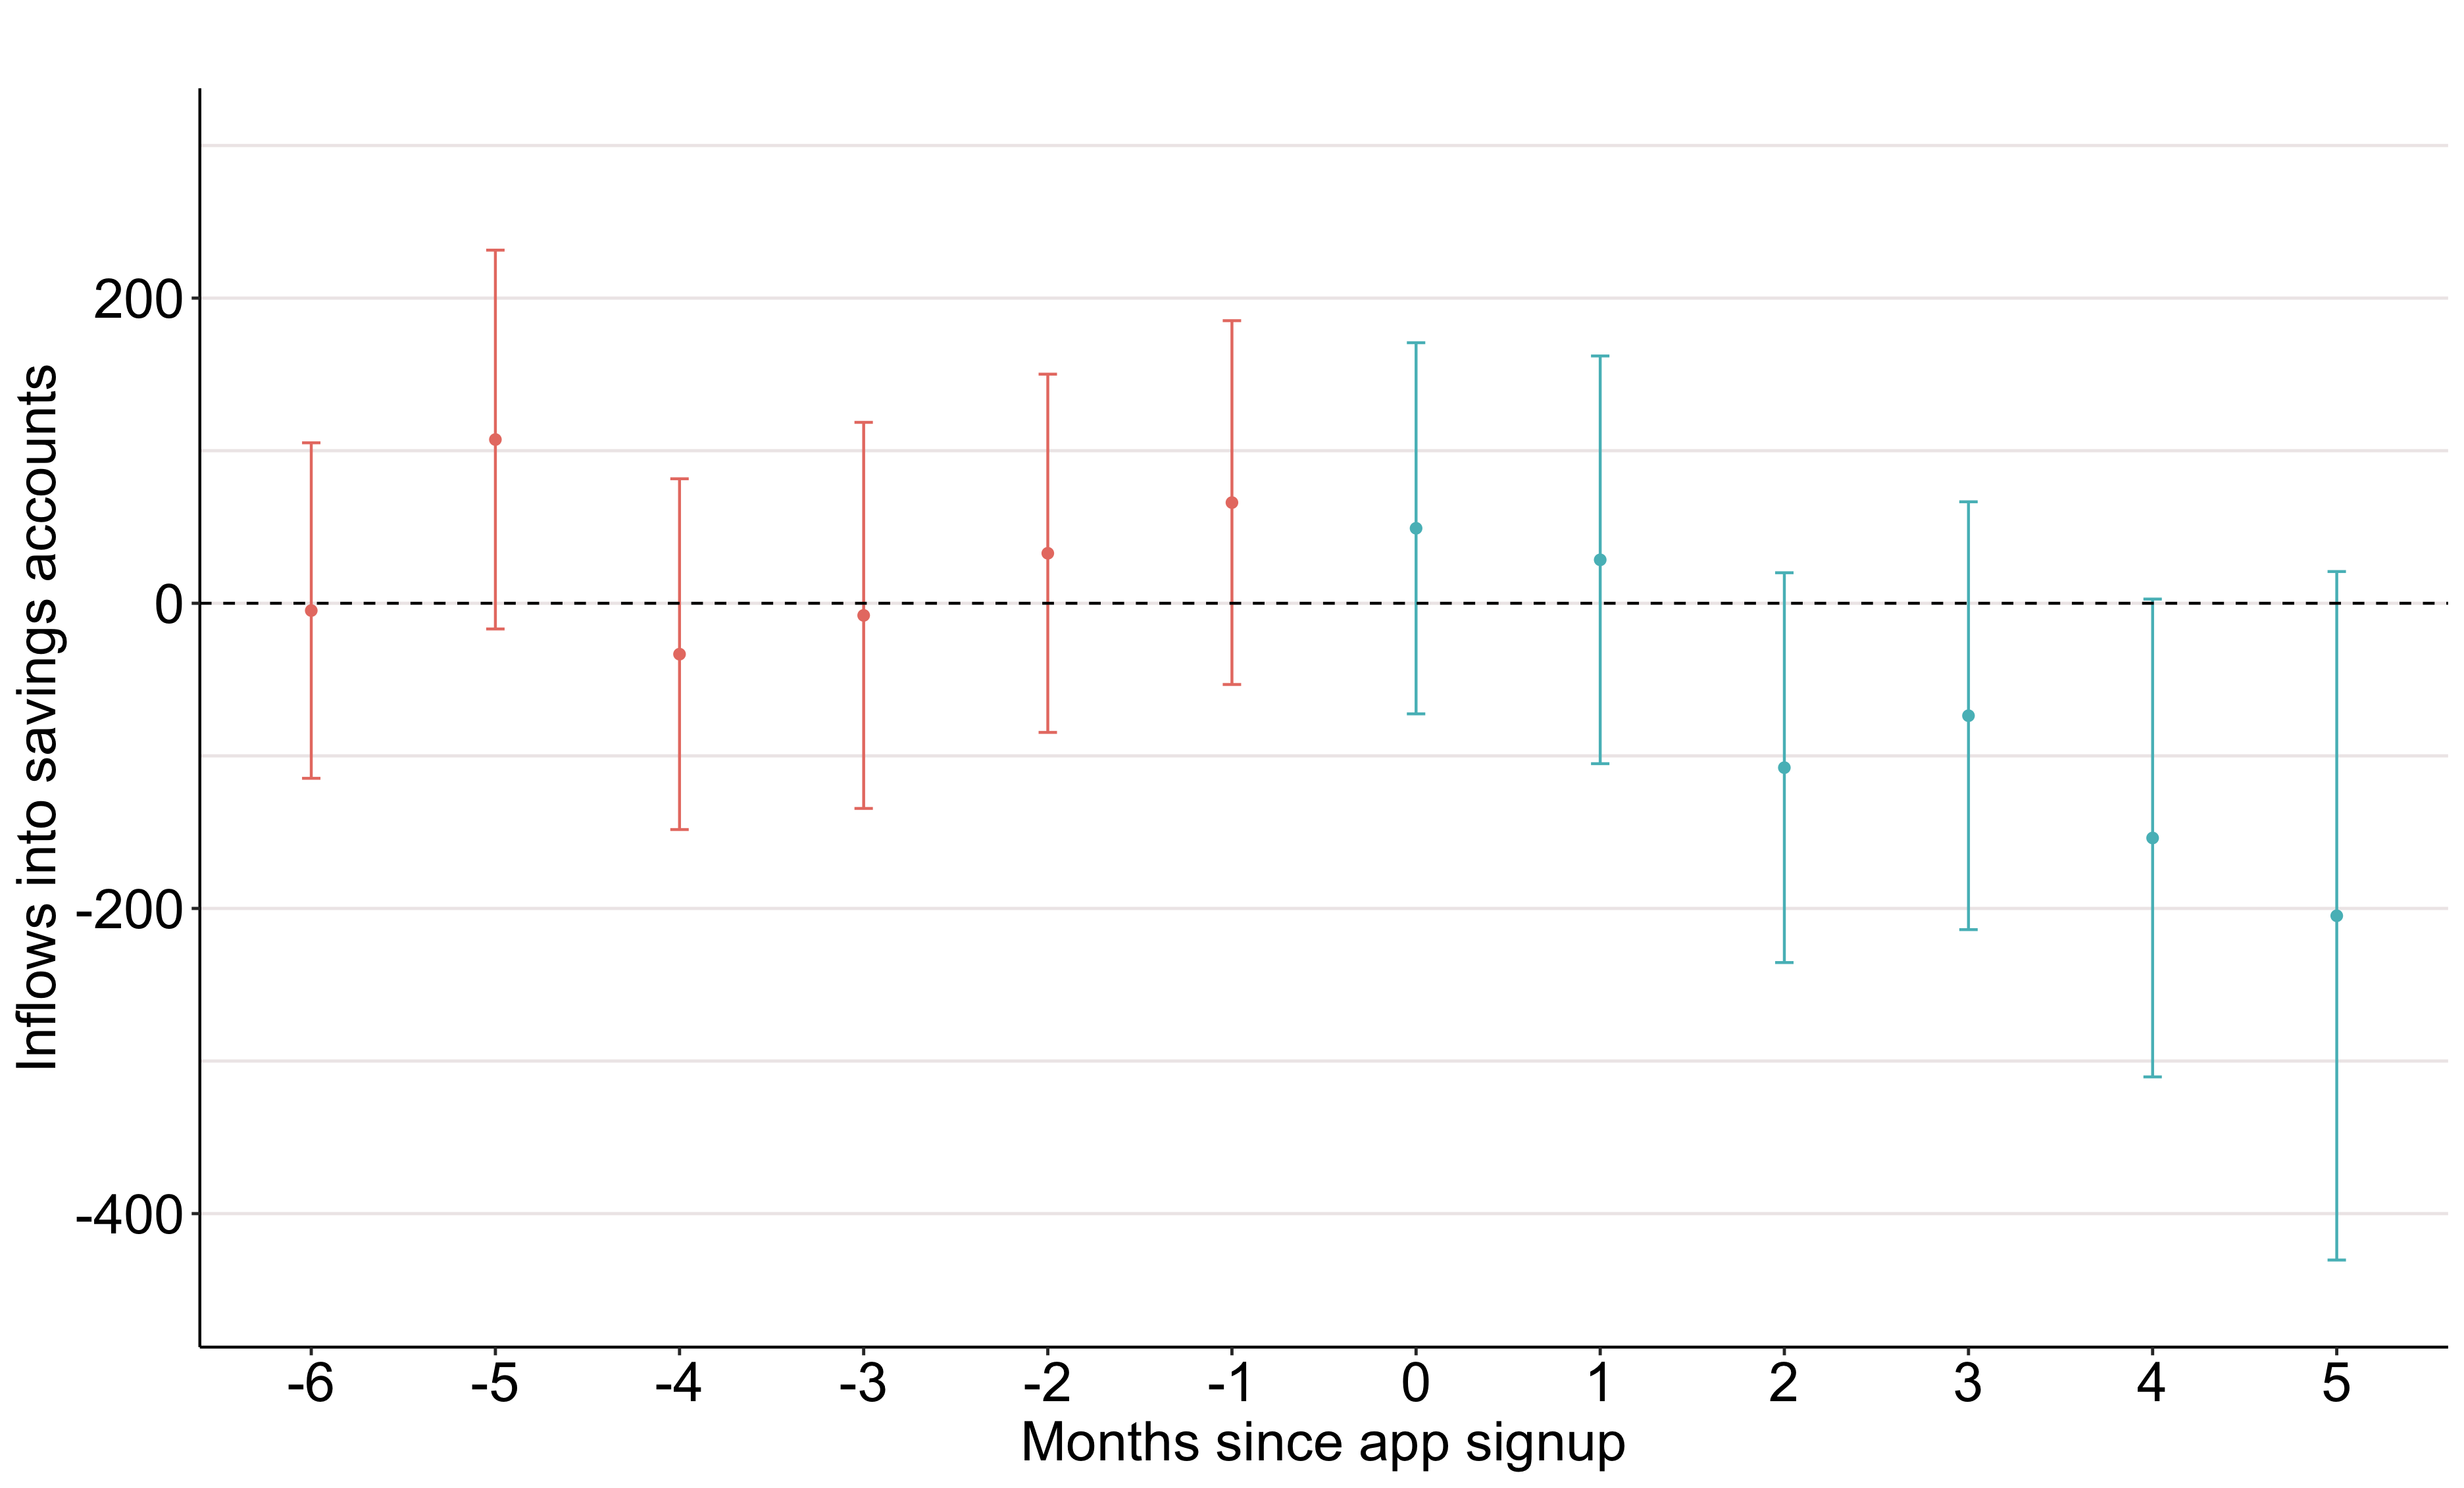
\includegraphics[width=.7\textwidth]{\figdir/inflows_cond_es.png}
    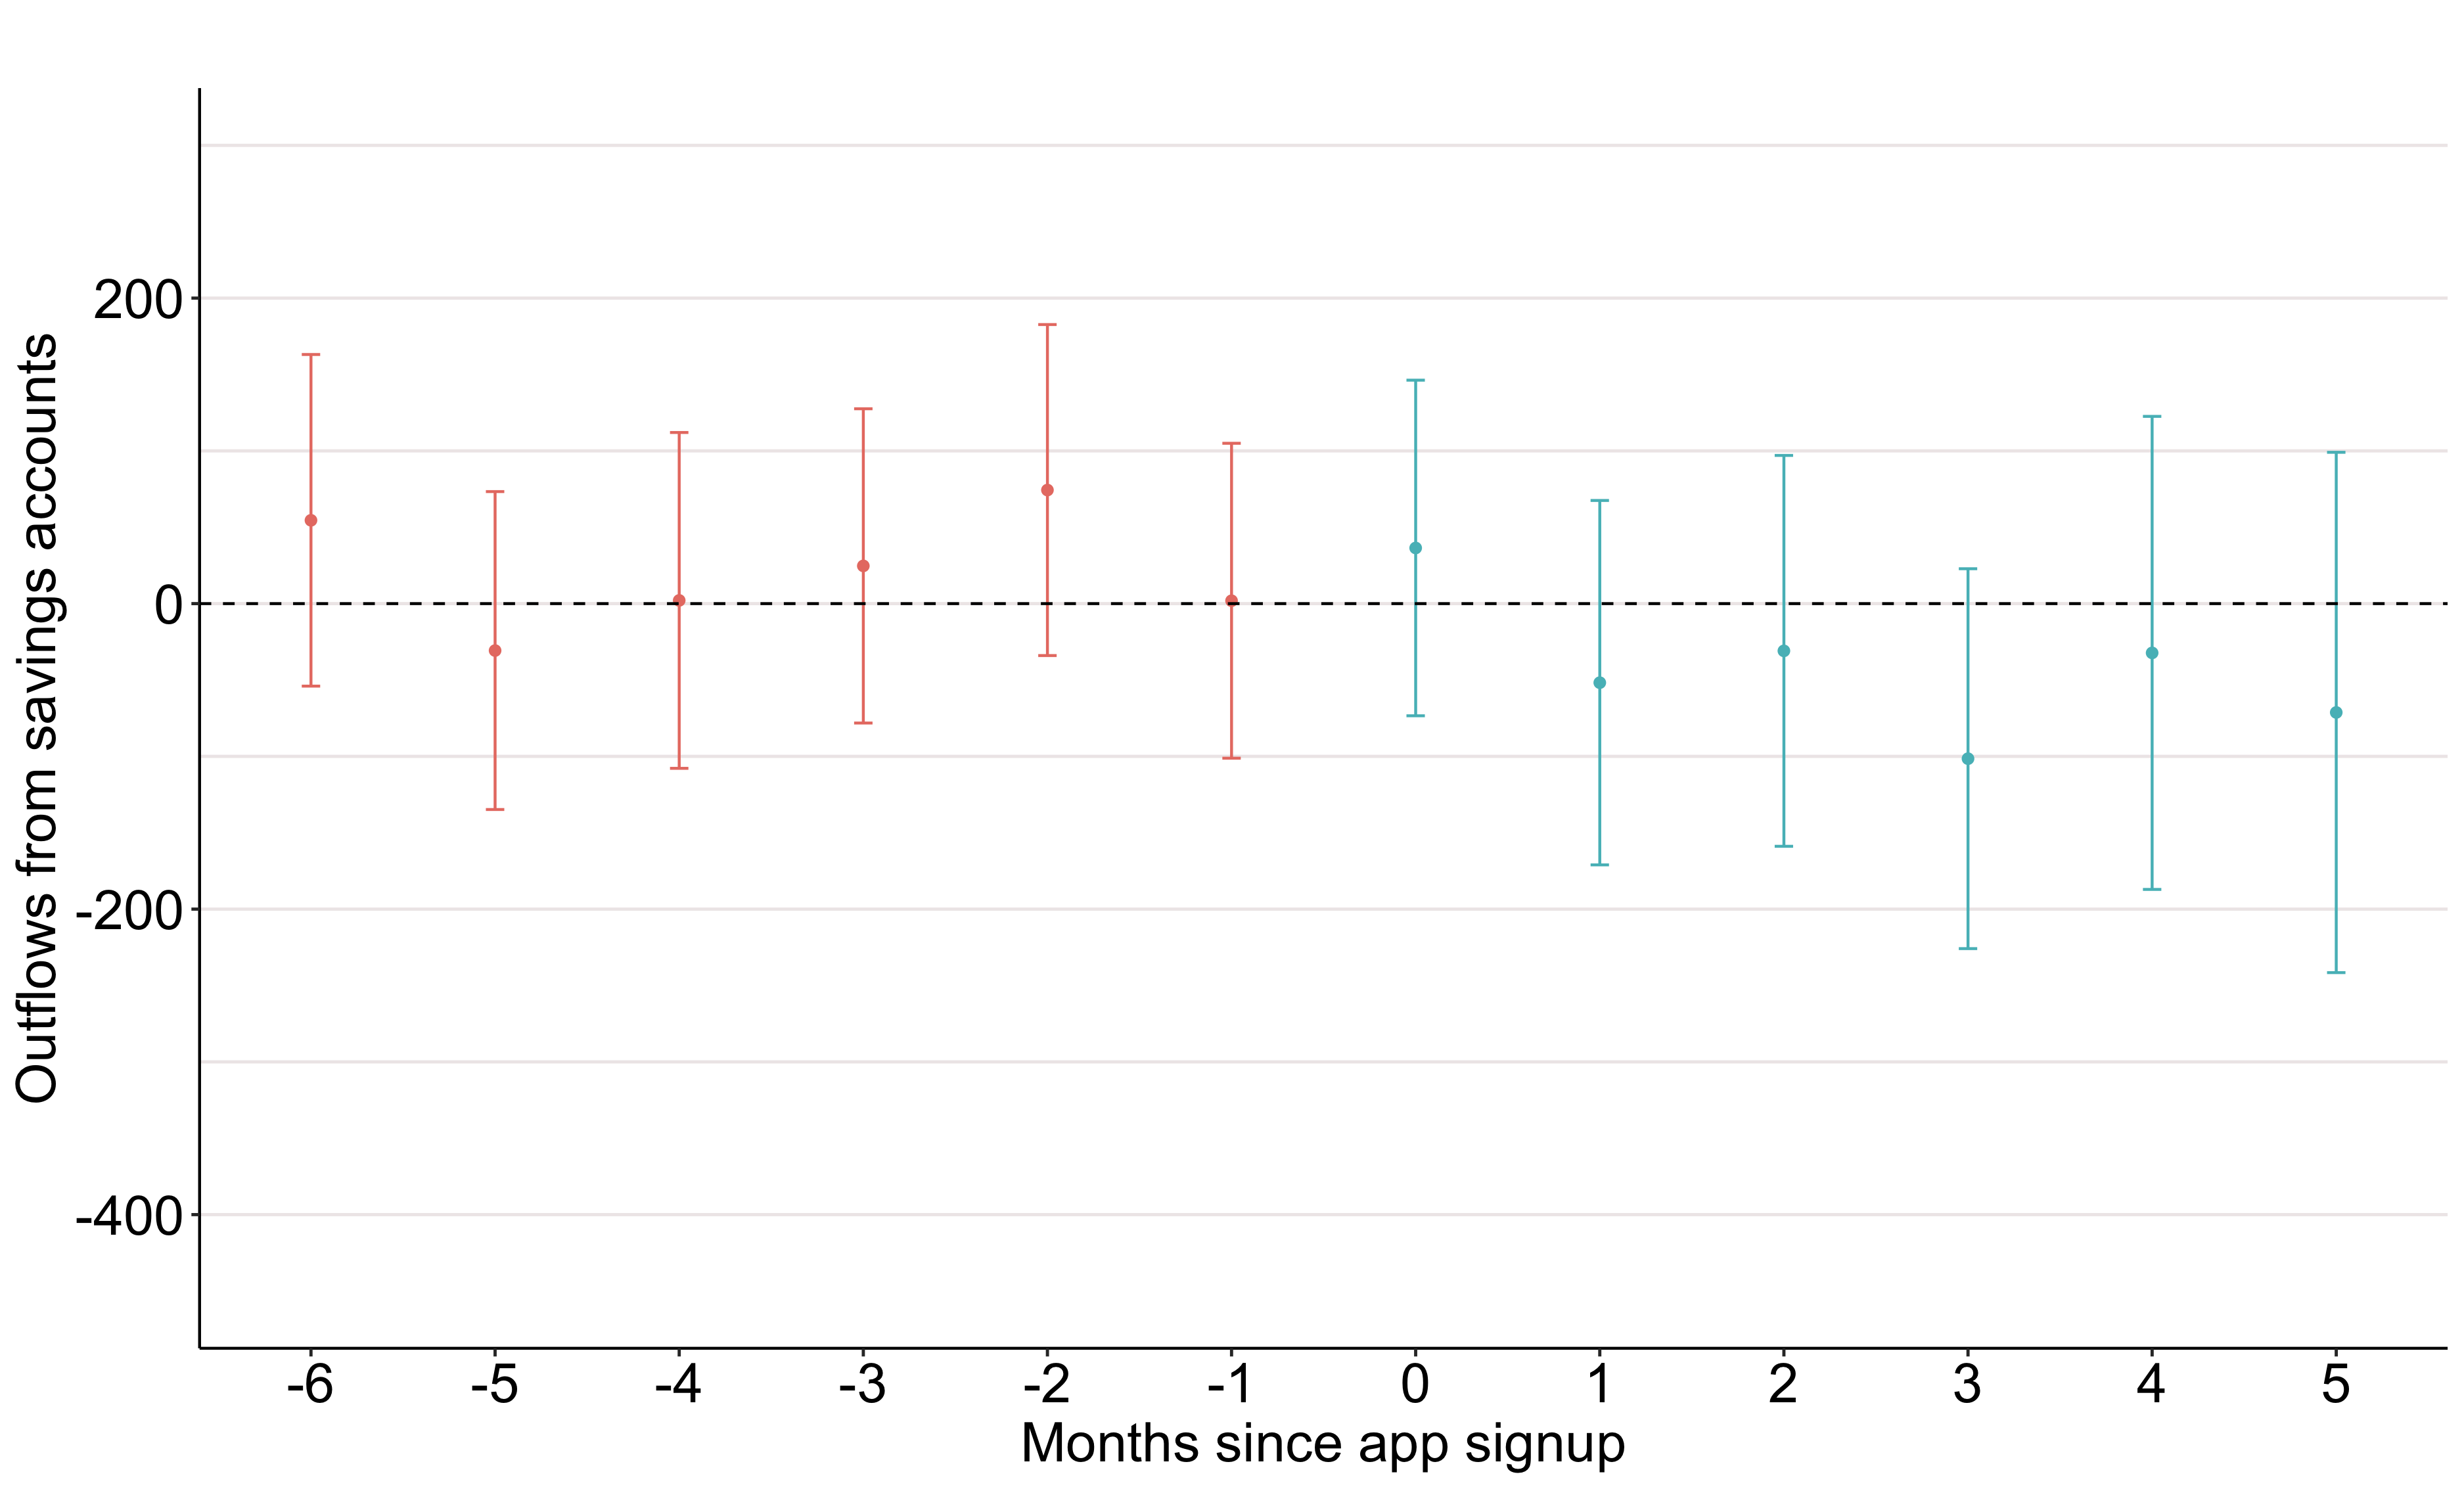
\includegraphics[width=.7\textwidth]{\figdir/outflows_cond_es.png}
    \fignote{\textwidth}{Decomposition of net-inflows into savings accounts
        (top) into inflows (middle) and outflows (bottom). Point estimates
        represent group-time average treatment effects aggregated to periods
        since treatment exposure, as defined in Section~\ref{sec:estimation}.
        Red lines represent point estimates and uniform 95\% confidence bands
        for pre-treatment periods allowing for clustering at the user level. If
        the null hypothesis that parallel trends hold in all periods is
        correct, these should be equal to zero. Blue lines provide similar
        information for post-treatment periods.}
\end{figure}

